In diesem Kapitel soll der experimentelle Aufbau des gesamten Lasersystems und
dessen Kopplung an die Vakuumapparatur mit dem Quadrupolmassenspektrometer
beschrieben werden.
Zunächst wird ein Überblick über das gesamte System gegeben (Abschn.
\ref{sec:gesamtaufbau}). Abschnitt \ref{sec:lasersystem} beschriebt den
optischen Aufbau inklusive Laserstabilisierung. Die Weiterverarbeitung der
Laserinformation und die Stabilisierung sollen in Abschn.
\ref{sec:elektronik_laserkontrolle} genauer betrachtet werden. In Abschn.
\ref{sec:vakuumapparatur_qms} und \ref{sec:messdatenverarbeitung} wird kurz
auf die verwendete Vakuumapparatur mit Quadrupolmassenspektrometer (QMS) und die
Messdatenverarbeitung eingegangen.
Abschnitt \ref{sec:vergleich_mit_altem_system} gibt einen kurzen Vergleich mit dem
bisher verwendeten, alten System.

\section{Gesamtaufbau}\label{sec:gesamtaufbau}
\begin{figure}[h]
 	\centering
 	\fbox{\parbox{\dimexpr \linewidth - 2\fboxrule - 2\fboxsep}{
 	\centering
	    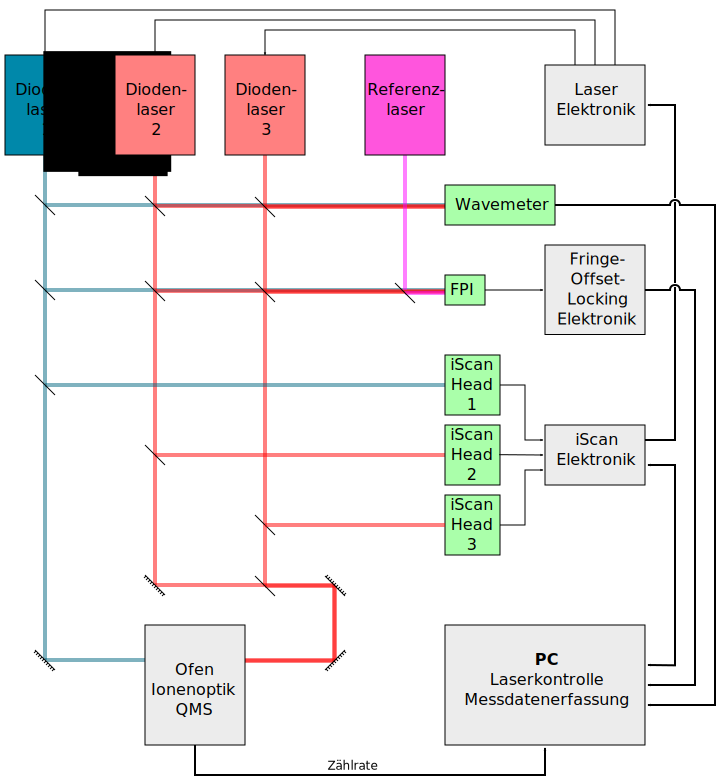
\includegraphics[width=\textwidth-2cm]{gfx/experimenteller_aufbau_gesamt}
	}}
	\caption[Gesamter experimenteller Aufbau, schematisch]{Dargestellt ist
	schematisch der gesamte experimentelle Aufbau des
	Systems.}\label{fig:experimenteller_aufbau_gesamt}
\end{figure}
Abbildung \ref{fig:experimenteller_aufbau_gesamt} zeigt schematisch den
Aufbau des gesamten Systems für den laserspektrometrischen Ultraspurennachweis.
Das zur resonanten Anregung benötigte Licht wird mit drei Diodenlasern erzeugt. Der größte Teil des Lichts wird
direkt in die Vakuumapparatur geführt. Letztere enthält einen Ofen für das
Ausheizen der Atome, die Ionenoptik für den Transport der erzeugten Ionen und
den Quadrupolmassenfilter zur Massenselektion der Ionen.
Die Einstrahlung der Laser erfolgt aus den in Abschn. \ref{sec:linienprofil}
erläuterten Gründen transversal zum aus dem Ofen austretenden kollimierten Atomstrahl.
Abgriffe der Hauptstrahlen führen das Laserlicht eines jeden Lasers in ein
Wavemeter, welches die Absolutwellenlängen liefert und an einen PC weiterleitet.
Jeweils zwei weitere Abgriffe führen die Strahlen in die Optiken von
\textit{iScan head} und FPI der zwei verwendeten Laserstabilisierungen. Die dort erzeugten
Signale werden an die jeweilige Elektronik weitergeleitet. Die Steuerung eines
\textit{iScan heads} ist die \textit{iScan control unit}, die direkt an die
Elektronik des entsprechenden Lasers angeschlossen ist und sowohl die Spannung
des Piezoaktuators des Laserresonators als auch den Strom der Laserdiode
moduliert.
Die Elektronik für das FOL bereitet die analogen Signale des FPIs digital auf und
leitet sie weiter an den PC, der gleichzeitig mit den \textit{iScan control units} bidirektional
verbunden ist und die Regelung der \textit{iScan}-Sollwerte übernimmt. Weiterhin
kann mit dem PC die Zählrate der Ionen, die einzeln durch ein hinter dem QMS
angebrachten Ionendetektor nachgewiesen werden, aufgenommen werden. Die
Steuerung des Massenspektrometers bezüglich der Einstellung sowie des Scans
bestimmter Massen durch den PC wurde im Rahmen dieser Arbeit noch nicht realisiert, soll aber
nachfolgend implementiert werden. Statdessen wird hierfür bis zum Abschluss
dieser Arbeit noch ein PC des Vorgängersystems verwendet.

\section{Lasersystem}\label{sec:lasersystem}
\begin{figure}[h]
 	\centering
 	\fbox{\parbox{\dimexpr \linewidth - 2\fboxrule - 2\fboxsep}{
 	\centering
	    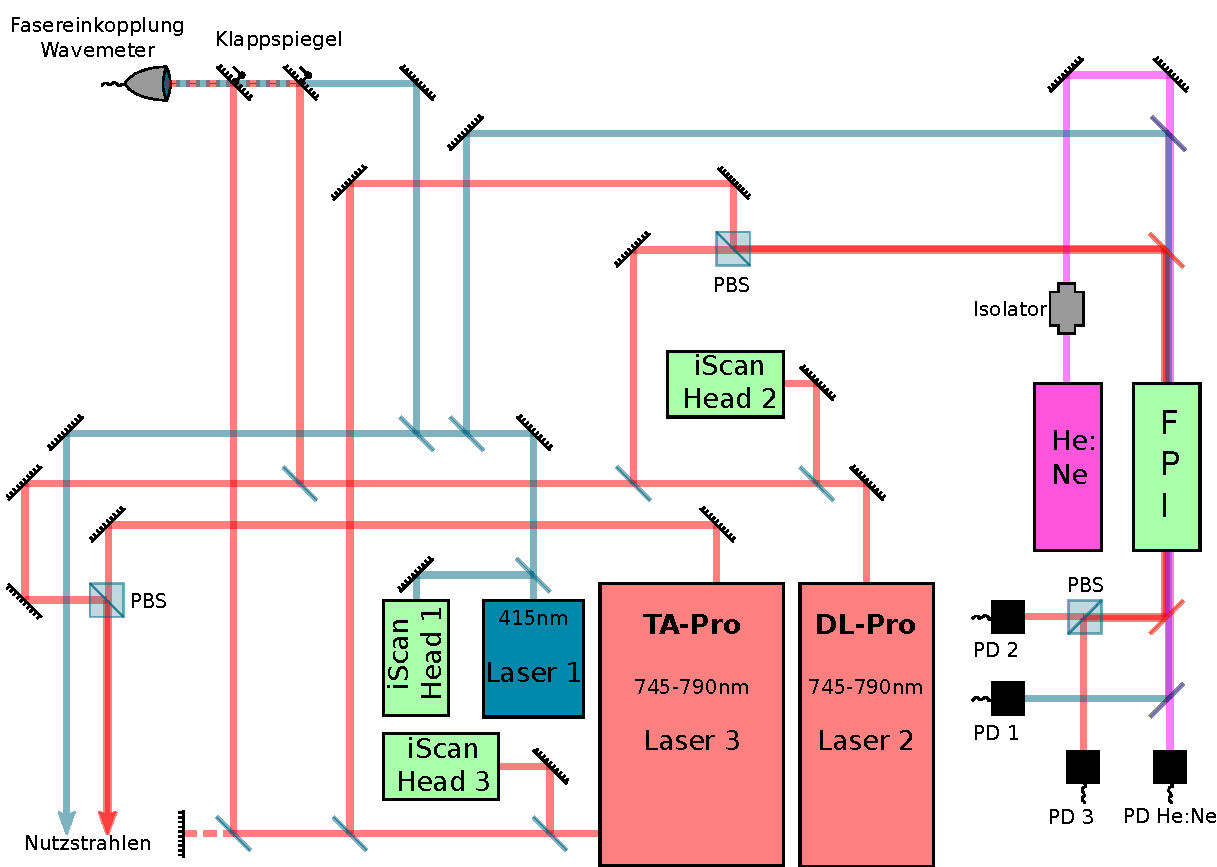
\includegraphics[width=\textwidth-2cm]{gfx/experimenteller_aufbau_lasersystem}
	    }}
	\caption[Experimenteller Aufbau des Lasersystems, schematisch]{Dargestellt ist
	schematisch der experimentelle Aufbau des
	Lasersystems.}\label{fig:experimenteller_aufbau_lasersystem}
\end{figure}
\begin{figure}[h]
 	\centering
 	\fbox{\parbox{\dimexpr \linewidth - 2\fboxrule - 2\fboxsep}{
 	\centering
	    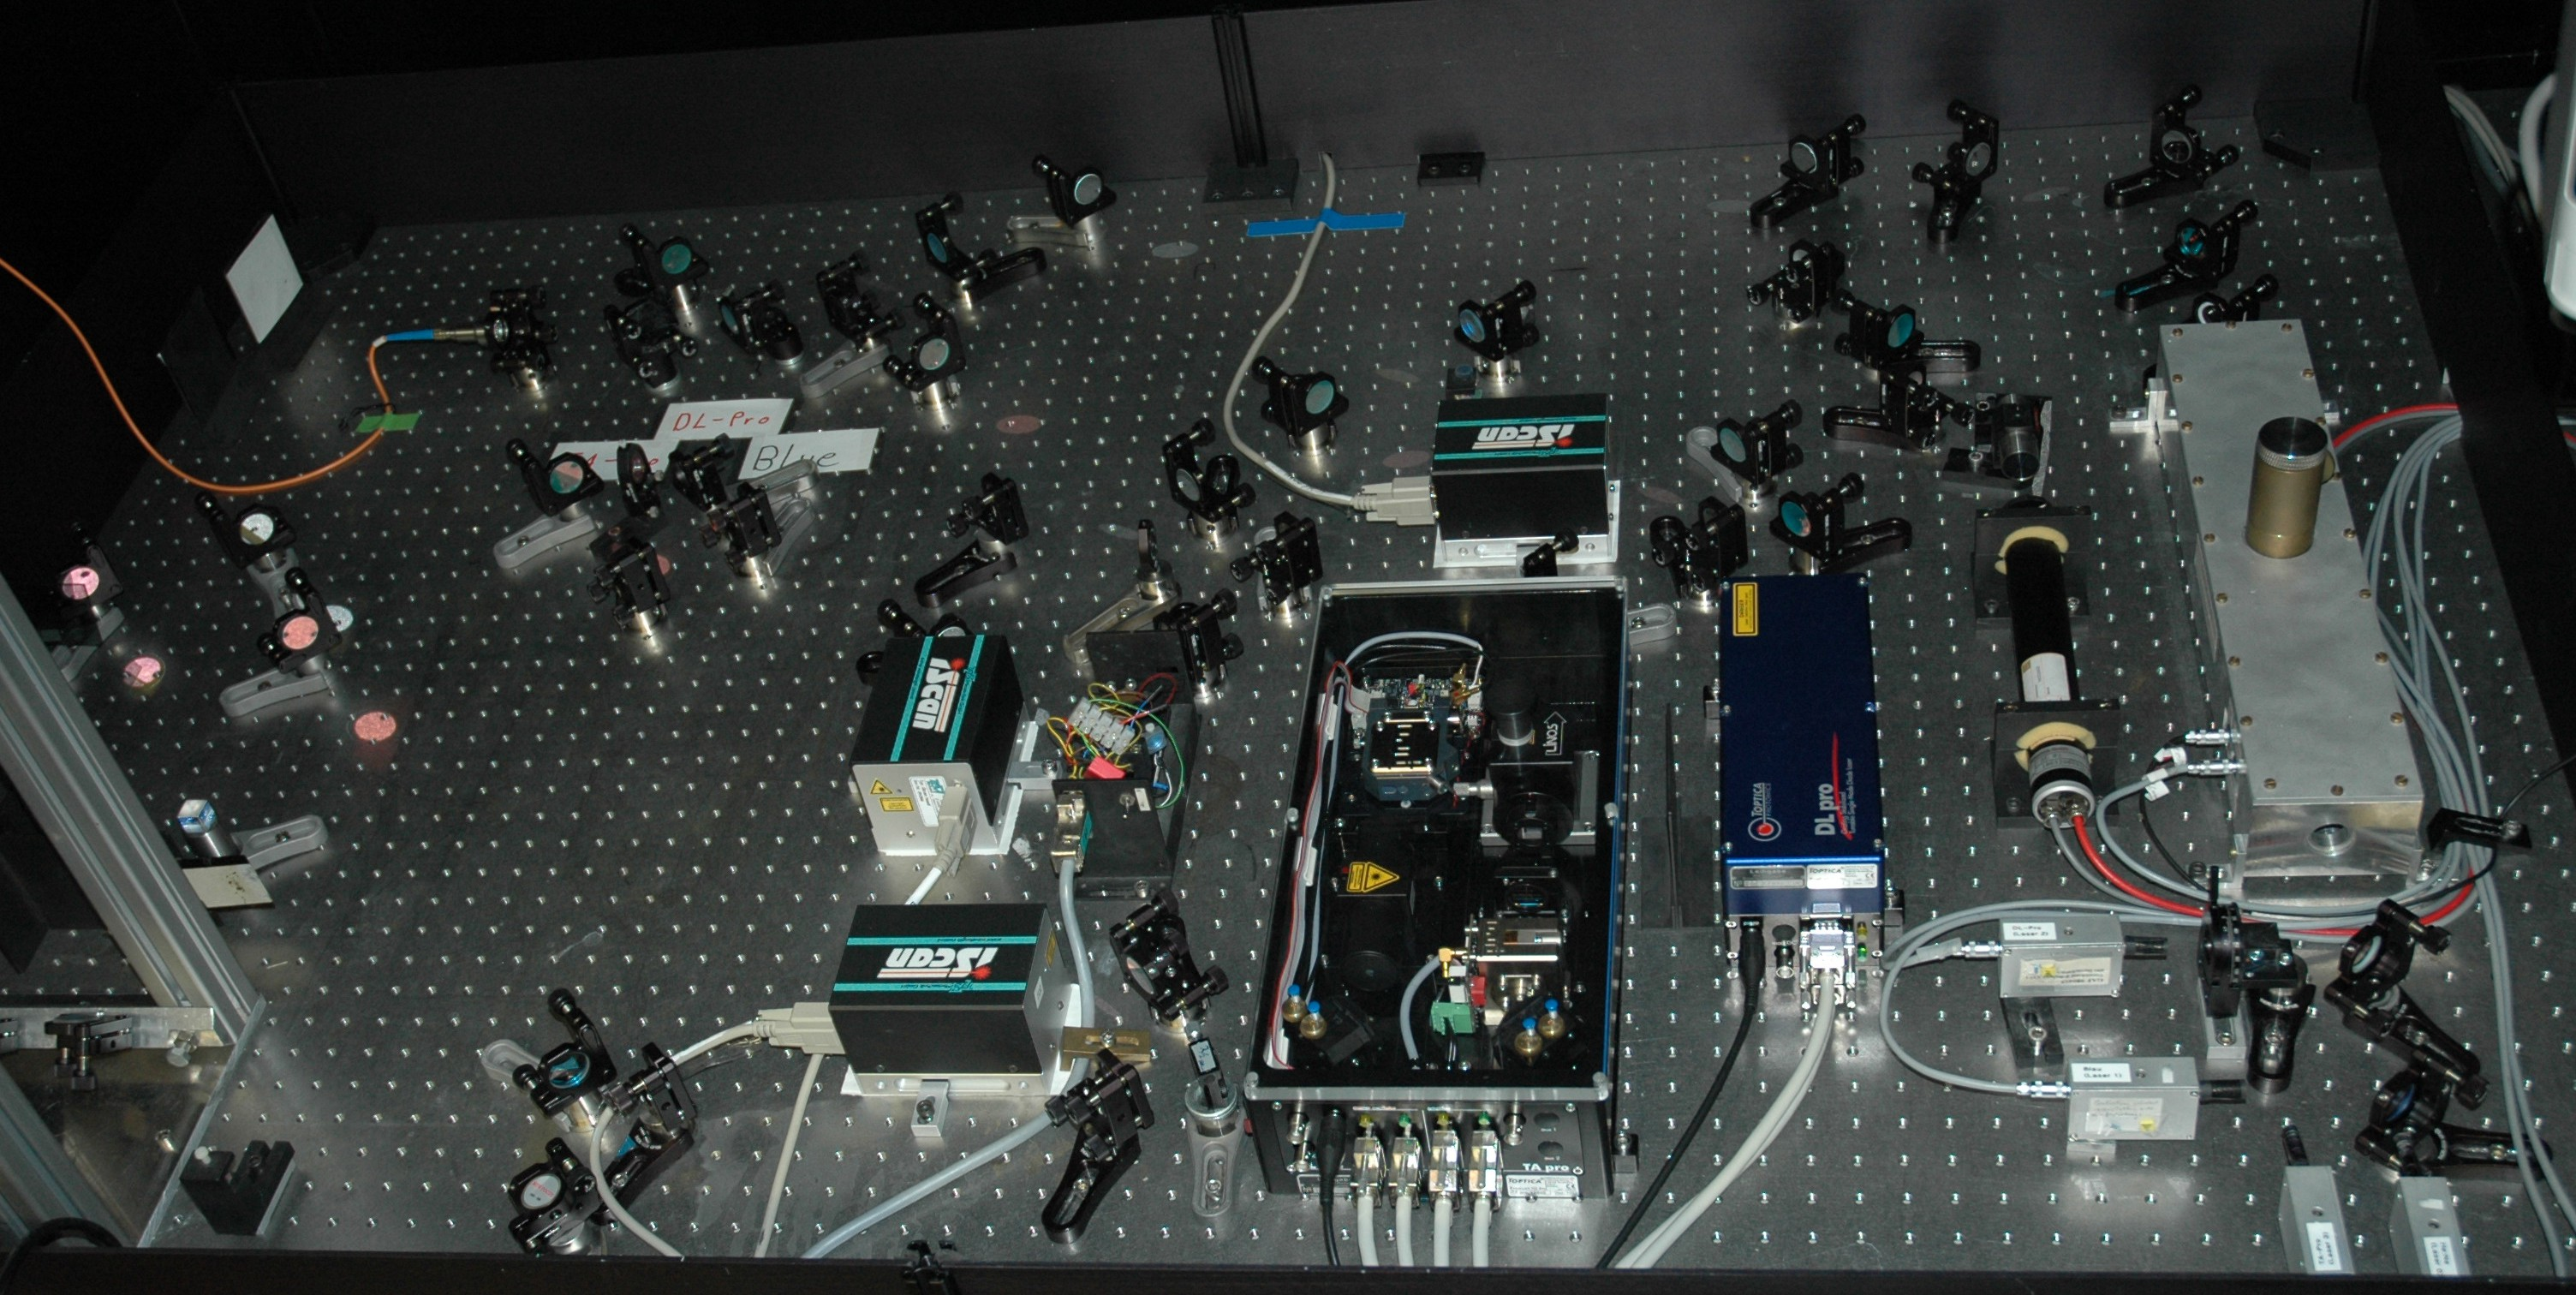
\includegraphics[width=\textwidth-0.5cm]{gfx/experimenteller_aufbau_lasersystem_foto}
	    }}
	\caption[Experimenteller Aufbau des Lasersystems -
	Foto]{Das Foto zeigt das verwendeten Lasersystems. Eingezeichnet sind die
	Strahlengänge der Laser.}\label{fig:experimenteller_aufbau_lasersystem_foto}
\end{figure}
Ein detaillierter Aufbau des Lasersystems wird schematisch durch Abb.
\ref{fig:experimenteller_aufbau_lasersystem} veranschaulicht und ist als
Fotografie in Abb. \ref{fig:experimenteller_aufbau_lasersystem_foto} noch einmal
zu sehen.\par
\begin{figure}[h]
 	\centering
 	\fbox{\parbox{\dimexpr \linewidth - 2\fboxrule - 2\fboxsep}{
 	\centering
	    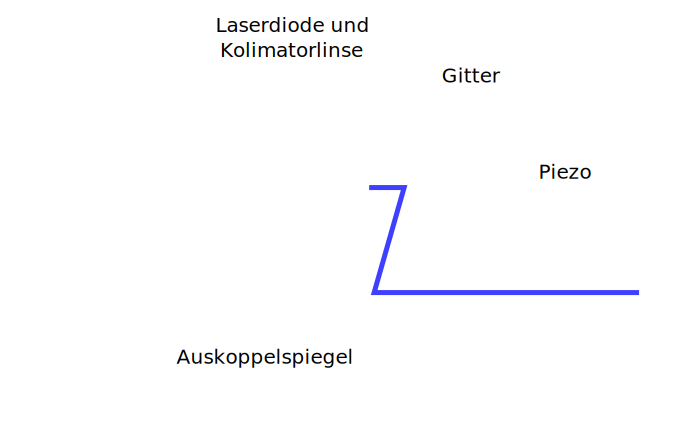
\includegraphics[width=\textwidth-1cm]{gfx/experimenteller_aufbau_diodenlaser_foto}
	    }}
	\caption[Diodenlaser - Foto]{Das Foto zeigt den Diodenlaser mit
	$405\,$nm-Diode und externen
	Resonator (Laser für den ersten
	Anregungsschritt).
	Eingezeichnet sind
	Laserdiode mit Kolimator,
	Gitter, Piezo,
	Auskoppelspiegel und
	Strahlengangd des
	Laserlichts.}\label{fig:experimenteller_aufbau_diodenlaser_foto}
\end{figure}
Das Laserlicht für den ersten Anregungsschritt wird in einem nach dem
Littrow-Design gebauten Diodenlaser erzeugt. Eingebaut ist eine blaue
$405\,$nm-Laserdiode mit einer Verstärkungsbandbreite von $\pm1\,$nm bei
zugeschaltetem externem Resonator (siehe Abb.
\ref{fig:experimenteller_aufbau_diodenlaser_foto}). Der modensprungfreie
Verstimmungsbereich ist mit $15\,$GHz spezifiziert. In einigen Moden wurden
allerdings auch Verstimmungsbreite von bis zu $20\,$GHz erreicht. Das Laserlicht
des zweiten und dritten Anregungsschritts wird mit zwei kommerziellen, ebenfalls im Littrow-Design gebauten, Diodenlasern der Firma \textit{Toptica} erzeugt.
Beide verwendeten Laserdioden haben ein spezifiziertes Verstärkungsprofil von
$745$ bis $790\,$nm und einen modensprungfreien Verstimmungsbereich von bis
zu $30\,$GHz, was experimentell bestätigt wurde. Weiterhin kann das Laserlicht
der Diode für den dritten Anregungsschritt mit einem Trapezverstärker wahlweise bis auf eine
Leistung von $1,5\,$W verstärkt werden. Neben dem leistungsstarken Nutzstrahl
gibt es bei diesem Ansatz noch die Möglichkeit, einen Teil des zum
Injection-Seeding verwendeten Masterlaserstrahls abzugreifen (links unten am TA-Pro in Abb.
\ref{fig:experimenteller_aufbau_lasersystem}). Für den ersten bzw.
zweiten Anregungsschritt können ca. $7\,$mW bzw. ca. $60\,$mW bei Diodenströmen von ca. $35\,$mA bzw. ca.
$120\,$mA erreicht werden, was für die Untersuchung von Uranisotopen vollkommen
ausreichend ist. Die Sättigungsleistungen werden im ersten Schritt bei $<1\,$mW,
im zweiten Schritt bei wenige mW und im dritten Schritt bei wenige $100\,$mW
vermutet.
Tabelle \ref{tab:laser_spezifikationen} listet noch einmal alle Laser-Spezifikationen auf.
%TODO: !!Referenz zu Lasermanuals / Diodenmanuals
%TODO: !!Laserspecs
\par
\begin{table}
	%Summe der Breiten muss 0.91 mal \textwidth sein.
	\begin{tabular}{p{0.23\textwidth}|p{0.24\textwidth}p{0.24\textwidth}p{0.24\textwidth}}
		\toprule
		& Laser 1 & Laser 2 & Laser 3\\
		\midrule[1px]
		\hline
		Bezeichnung & Eigenbau & DL-Pro & TA-Pro\\
		Wellenlänge & $405\pm1\,$nm & $745\,$-$790\,$nm & $745\,$-$790\,$nm\\
		max. Leistung & $7\,$mW & $60\,$mW & $1,5\,$W\\
		nötige Leistung & $<1\,$mW* & wenige mW* & wenige $100\,$mW*\\
		Externer Resonator & Littrow & Littrow & Littrow\\
		\bottomrule[1px]
	\end{tabular}
	\caption[Spezifikationen der verwendeten
	Diodenlaser]{Aufgelistet sind die Spezifikationen der verwendeten
	Diodenlaser.\\
	*: vermutete Werte, Sättigungsmessungen müssen noch durchgeführt werden.}
	\label{tab:laser_spezifikationen}
\end{table}
Die Teilstrahlen für die Stabilisierung der \textit{iScans} werden aufgrund der
in \ref{subsec:iScan} erklärten Empfindlichkeit auf räumliche Drifts auf
möglichst kurzem Weg in die \textit{iScan heads} geführt, um die Hebelwirkung
bei Drifts möglichst klein zu halten. Die Polarisation von Laser 3 muss für
das \textit{iScan} und die Überlagerung mit dem Strahl von Laser 2 mit einem
$\nicefrac{\lambda}{2}$-Plättchen gedreht werden.\par
Die Abgriffe für das Wavemeter des Typs \textit{WS Ultimate} von der Firma \textit{High Finesse}
müssen mit Klappspiegeln einzeln ausgewählt werden, da immer nur das Licht eines Lasers im Wavemeter analysiert werden kann. Da das Wavemeter eine
Absolutgenauigkeit von $40\,$MHz hat
\cite{wavemeter_hardware_guide}, würde es zur Frequenzstabilisierung nicht
genügen, ist aber für das Finden von Resonanzen und, wie schon erwähnt, zum
Berechnen der Relativfrequenzen nach Gl. \eqref{eq:FPI_frequenzdrift_03} ausreichend.\par Für das FOL muss das Licht aller drei zu stabilisierenden
Laser vor dem FPI zusammengeführt und danach wieder getrennt werden. Da die
Wellenlängen von Laser 2 und 3 sehr nahe beieinander liegen, muss das Licht
dieser Laser mit Polarisationsstrahlteilern zusammengeführt und getrennt werden.
Dabei ist zu beachten, dass die Verluste durch die jeweils falsche Polarisation
der Laser möglichst gering sind, was durch optionales Drehen der
Polarisation mit $\nicefrac{\lambda}{2}$-Plättchen möglich ist. Die Überlagerung
mit dem blauen Licht des ersten Lasers und dem des He:Ne-Lasers kann mit
dichroitischen Spiegeln realisiert werden. Diese sind dafür ausgelegt, Licht
bestimmter Wellenlängenbereiche zu reflektieren, während Licht anderer  Bereiche
transmittiert wird. Die Trennung der Strahlen erfolgt nach demselben Prinzip.
Hinter dem gerampten FPI wird das Fringepattern aller vier Laser getrennt mit
Photodioden aufgenommen. Der FSR des FPIs wurde auf $(298,0856\pm0,0026)\,$MHz
bestimmt (siehe Abschn. \ref{sec:charakterisierung_FPI}).
Es ist zwecks Unterdrückung der Schwankungen des Brechungsindexes evakuiert,
wodurch $n_r\approx1$ gilt. Im nah-infraroten Bereich hat es die größte Finesse, wohingegen im blauen Bereich
die Finesse sehr schlecht ist. Das FOL ist damit zwar noch
möglich, es wird allerdings angestrebt, ein anderes Interferometer zu verwenden.
Dieses wird momentan noch in dem parallel laufenden alten System verwendet, das
während dem Entstehen dieser Arbeit noch als Referenzsystem eingesetzt und in
\ref{sec:vergleich_mit_altem_system} kurz beschrieben wird.\par
Die Hauptstrahlen werden an ein Periskop geführt, über das das Licht in einen
anderen Raum an die Vakuum-Apparatur transportiert wird, wobei das Licht von
Laser 2 und 3 durch Polarisationstrennung überlagert wird. Der
Strahltransport über das Periskop ist Teil einer vorübergehenden Lösung, da auf
dem Lasertisch bei der Vakuum-Apparatur noch das alte Lasersystem aufgebaut
ist.\par Der He:Ne-Laser ist gegen Rückreflexe aus dem FPI durch einen optischen Isolator
geschützt. Ebenso hat der dritte Laser vor dem Masterlaserabgriff und nach dem
Trapezverstärker je einen Isolator. Laser 1 und 2 haben momentan noch keinen
Isolator. Es soll jedoch in Zukunft jeweils ein Isolator zwischengeschaltet
werden. Weitere optische Aufbauten, für die in Fig.
\ref{fig:experimenteller_aufbau_lasersystem_foto} keine Strahlengänge eingezeichnet
sind, dienen der separaten Überlagerung der Strahlen beider roten Laser zur
Messung von Schwebungsfrequenzen (siehe Kap. \ref{kap:charakterisierung}).

\section{Elektronik der Laserkontrolle}\label{sec:elektronik_laserkontrolle} In
diesem Abschnitt wird die Verarbeitung der Signale zur Laserkontrolle schematisch erklärt. Für
Schaltpläne und interne elektronische Abläufe verschiedener Komponenten sei auf
den Anhang verwiesen. Abbildung \ref{fig:experimenteller_aufbau_elektronik_laserkontrolle} zeigt den
schematischen Aufbau der Elektronik für die Laserkontrolle.\par
\begin{figure}[h]
 	\centering
 	\fbox{\parbox{\dimexpr \linewidth - 2\fboxrule - 2\fboxsep}{
 	\centering
	    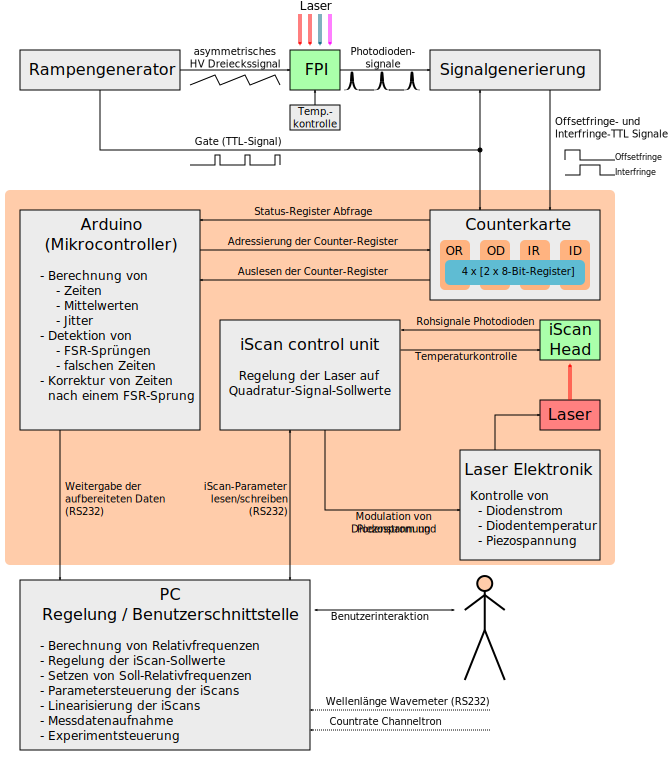
\includegraphics[width=\textwidth-2cm]{gfx/experimenteller_aufbau_elektronik_laserkontrolle}
	    }}
	\caption[Experimenteller Aufbau der Laserkontollelektronik,
	schematisch]{Es ist schematisch der experimenteller Aufbau der Elektronik der
	Laserkontrolle 
	dargestellt.}\label{fig:experimenteller_aufbau_elektronik_laserkontrolle}
\end{figure}

\subsection{Signalgenerierung}\label{subsec:signalgenerierung}
Das FPI wird durch einen Rampengenerator in seiner Länge linear durchgefahren.
Dazu wird ein asymmetrisches Dreieckssignal mit ca. $60\,$Hz erzeugt, welches
das wie in Abb.
\ref{fig:FPI_signal-zeitverlauf}(b) gezeigte Fringepattern für jeden Laser
an den Photodioden hinter dem FPI erzeugt. Außerdem gibt der Rampengenerator
ein TTL-Signal aus, das bei fallender Spannungsflanke HIGH und bei
steigender Spannungsflanke LOW ist. Die fallende bzw. steigende Flanke dieses
\textit{Gates} signalisiert also den Start bzw. das Ende der Spannungsrampe
und wird als Triggersignal verwendet. Die Photodiodensignale und das
Gate werden an einen Signalgenerator weitergegeben, welcher über Ableiten der
Fringesignale die wie in \ref{fig:FPI_signal-zeitverlauf}(d,e) gezeigten TTL-Pulse erzeugt.
Wie dies genau geschieht wird in Anh.
\ref{anh:sec:signalgenerierung_elektronik} beschrieben. Es ist weiterhin
möglich, einen \textit{Delay} in der Detektion des ersten Fringes einzustellen,
damit Nichtlinearitäten zu Beginn der Rampe umgangen werden.\par
Der im Folgenden beschriebene Ablauf ist für jeden zu stabilisierenden Laser
gleich (orange hinterlegter Bereich in Abb.
\ref{fig:experimenteller_aufbau_elektronik_laserkontrolle}). Daher wird dieser
Teil exemplarisch für einen Laser und den Referenzlaser beschrieben.

\subsection{Counterkarte}\label{subsec:counterkarte}
Die durch den Offsetfringe und Interfringe erzeugten
TTL-Pulse des zu stabilisierenden Lasers als auch des Referenzlasers
sowie das Gate werden an eine Counterkarte weitergeleitet. Diese besteht aus
vier 16-Bit-Countern und einem Taktgeber mit einstellbarer Taktrate ($1,25\,$MHz,
$2,5\,$MHz, $5\,$MHz und $10\,$MHz), wodurch unterschiedliche Zeitauflösungen möglich
sind ($0,8\,$\textmu s, $0,4\,$\textmu s, $0,2\,$\textmu s und $0,1\,$\textmu
s).
Wird das Gate auf LOW gesetzt (Beginn der steigenden Spannungsflanke), werden
alle Counter freigeschaltet. Wenn die durch
das Delay etwas verzögerten TTL-Signale der Offsetfringes auf HIGH gesetzt werden, beginnen die
entsprechenden Counter der Offsetfringes (OR und OD) zu zählen. Beim Eintreten
der Offsetfringes werden diese Counter gestoppt und die Counter für die
Interfringezeiten gestartet (IR und ID). Auch diese werden beim Eintreten der
Interfringes gestoppt. Am Ende der steigenden Spannungsflanke wird das Gate auf
HIGH gesetzt und die Counter werden gesperrt. Beim Stoppen eines jeden Counters
liegen die Counterwerte in jeweils 2x8-Bit-Registern (\textit{Upper Byte} und \textit{Lower Byte}) vor und es wird jeweils ein
\textit{Status-Bit} gesetzt, welches Abrufbereitschaft der entsprechenden
Counterwerte signalisiert.\par
Die Status-Bits sind über ein \textit{Statusregister} auslesbar. Die
Adressierung der einzelnen Counterregister wird über einen \textit{Adressbus} mit vier Bits
gesteuert, dessen Kodierung in Tab. \ref{tab:adressbus_kodierung} aufgeschlüsselt ist.
\begin{table}
	%Summe der Breiten muss 0.91 mal \textwidth sein.
	\begin{tabular}{p{0.1\textwidth}p{0.1\textwidth}p{0.1\textwidth}p{0.1\textwidth}|p{0.51\textwidth}}
		\toprule
		Enable & Addr. 1 & Addr. 2 & Addr. 3 & Wirkung\\
		\midrule[1px]
		\hline
		L & - & - & - & Adressierung deaktiviert\\
		H & L & L & L & Lower Byte Offsetfringe Referenzlaser\\
		H & L & L & H & Upper Byte Offsetfringe Referenzlaser\\
		H & L & H & L & Lower Byte Interfringe Referenzlaser\\
		H & L & H & H & Upper Byte Interfringe Referenzlaser\\
		H & H & L & L & Lower Byte Offsetfringe Diodenlaser\\
		H & H & L & H & Upper Byte Offsetfringe Diodenlaser\\
		H & H & H & L & Lower Byte Interfringe Diodenlaser\\
		H & H & H & H & Upper Byte Interfringe Diodenlaser\\
		\bottomrule[1px]
	\end{tabular}
	\caption[Adressierung Counterregister]{Die Tabelle schlüsselt die Adressierung
	der Counterregister auf.}
	\label{tab:adressbus_kodierung}
\end{table}
Dabei sind \textit{Addr. 1}, \textit{Addr. 2} und \textit{Addr. 3} die
Adressleitungen. Über \textit{Enable} kann die Adressierung aktiviert und
deaktiviert werden. Sehr wichtig hierbei ist, dass bei einem Adressierungswechsel auf ein anderes
Counterregister die Adressierung immer deaktiviert werden muss. Andernfalls kann
es zur Zerstörung der Counter kommen. Schaltpläne und nähere Erläuterungen
zu der Counterkarte sind in Anh. \ref{anh:sec:counterkarte} zu finden.

\subsection{Datenaufbereitung (\textit{Arduino})}\label{subsec:arduino}
Die Auslese und Weiterverarbeitung der Werte muss nun bis spätestens zur
nächsten steigenden Spannungsrampe abgeschlossen sein, damit wieder die neuen
Rampensignale abgearbeitet werden können und es zu keinem Datenverlust kommt.
Dafür stehen der weiteren Datenverarbeitung im schlimmsten Fall nur $2\,$ms zur
Verfügung. Da bei einem PC mit klassischem Betriebssystem-Kernel wie Windows
NT$^\text{\textregistered}$ oder Linux die Prozessverwaltung aufgrund von
unvorhersehbaren Interrupts nie deterministisch ist, ist es sehr unsicher, die
Daten direkt mit einem PC zu verarbeiten. Daher werden die Daten zunächst von einem Mikrocontroller
aufbereitet, bevor sie weiter an einen PC gesendet werden. Ein Mikrocontroller
benötigt für gleiche Rechenvorgänge immer die gleiche Zeit, da es nie zu
unvorhergesehenen Interrupts kommen kann. Als Mikrocontroller eignet sich dafür
hervorragend die Entwicklungsplattform \textit{Arduino$^\text{\textregistered}$}\footnote{http://www.arduino.cc}. Diese
wird verwendet, da sich das Projekt seitens der Elektronik und Software
auch nach Abschluss dieser Arbeit noch in der Entwicklungsphase befindet und der
\textit{Arduino} durch eine USB-Schnittstelle für einen PC eine unkomplizierte
Handhabung und Programmierung bietet, was für Entwicklungszwecke gegenüber einem
einfachen Mikrocontroller-Chip ohne diese Perepherie vorteilhaft ist. Der hier eingesetzte
\textit{Arduino Mega 2560} mit dem Mikrocontroller-Chip \textit{ATmega2560}
bietet 54 digitale Ein- und Ausgänge. Er hat eine Taktrate von $16\,$MHz und
einen Flashspeicher von $256\,$kb für den binären Programmcode.
Die Programmierung erfolgt über eine frei verfügbare Entwicklungsumgebung.\par
Über das Statusregister erfährt der \textit{Arduino}, ob einer der Counter das Zählen
beendet hat, adressiert dessen Register und liest diese über einen
8-Bit-Datenbus aus. Nach dem Ende einer steigenden Rampe hat der
\textit{Arduino} im schlimmsten Fall noch maximal $2\,$ms Zeit, um abschließende Berechnungen
auszuführen. Die Aufgabe des \textit{Arduinos} ist es, die Zeiten $t_{OR}$,
$t_{OD}$, $t_{IR}$ und $t_{ID}$ zu berechnen und Mittelwerte über mehrer Rampenzyklen zu
bilden. Darüber hinaus wird der Laser-Jitter über mehrere Rampenzyklen
ermittelt, Sprünge in benachbarte FSRs des FPIs detektiert und Zeiten
korrigiert. Außerdem werden ungewöhnliche Zeiten verworfen. Wie dies genau
abläuft, soll in Kap. \ref{kap:software} erläutert werden. So geht möglichst
wenig Information über die Laser verloren, wobei gleichzeitig dem PC genügend
Zeit zur Verfügung steht, um die Regelung der \textit{iScan}-Sollwerte
abzuwickeln.

\subsection{PC: Regelung und
Benutzerschnittstelle}\label{subsec:pc_regelung_benutzerschnittstelle}
Die aufbereiteten Daten werden anschließend über eine RS232-Schnittstelle an einen mit Windows
7$^\text{\textregistered}$ aufgesetzten PC übermittelt, auf dem ein auf
\textit{Labview} basierendes Kontrollprogramm läuft. \textit{Labview} übernimmt nun die endgültige Berechnung der
Ist-Relativfrequenzen und die Regelung auf die eingestellte Soll-Relativfrequenz
aller drei Laser über das Setzen der \textit{iScan}-Sollwerte, wie schon in
Abschn.
\ref{sec:iscan_und_fringe-offset-locking} beschrieben wurde.
Dazu ist der PC wiederum über RS232-Schnittstellen an die \textit{iScan control
units} angeschlossen. Es entstehen zwar wegen der Mittelung der Werte durch den
\textit{Arduino} in wesentlich geringerer Rate Datenpakete für die Stabilisierung über den PC. Da
die Regelung über das FOL aber ohnehin nur zum Ausgleichen der Fehler und Drifts
der \textit{iScans} dient, ist diese etwas "`gemächlichere"' Regelung kein
Nachteil.
Weiterhin übernimmt das \textit{Labview}-Programm Monitoraufgaben der Laser,
Parametersteuerung der \textit{iScans}, Messdatenaufnahme, Experimentsteuerung
und Linearisierung der \textit{iScans}, was in Kap. \ref{kap:software}
detailierter erklärt wird.\par

\subsection{\textit{iScan control unit}}\label{subsec:iscan_control_unit}
Neben der Regelung der Laser auf einen Sollwert bietet die \textit{iScan control
unit} noch weitere Funktionen wie z.B. Frequenzscans und Datenaufnahme. Dieser
Abschnitt soll sich allerdings auf die Regelung der \textit{iScans} beschränken.
Weitere Funktionen werden z.B. bei der Linearisierung der \textit{iScans}
benutzt (siehe Abschn.
\ref{sec:linearisierung_iscan}).\par
Abbildung \ref{fig:iscan_control_unit_regelelektronik} zeigt schematisch den
Teil der Elektronik der \textit{iScan control unit}, der für die Regelung und
die Manipulation der Laserparameter zuständig ist. Die Peripherie-Elektronik und
detaillierte Schaltungen wurden dabei bewusst ausgelassen, um die Übersicht zu
bewahren. Für Detailschaltungen sei auf das Hardwarehandbuch der \textit{iScans}
verwiesen \cite{iscan_hardware_guide}.\par
\begin{figure}[h]
 	\centering
 	\fbox{\parbox{\dimexpr \linewidth - 2\fboxrule - 2\fboxsep}{
 	\centering
	    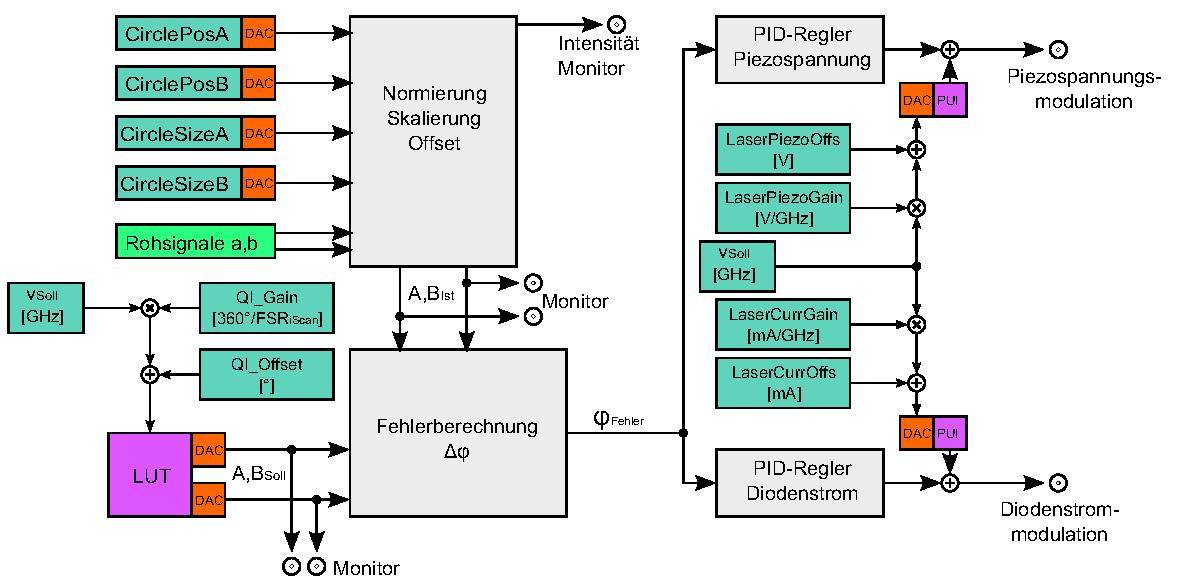
\includegraphics[width=\textwidth-0cm]{gfx/iscan_control_unit_regelelektronik}
	    }}
	\caption[Interner Aufbau der \textit{iScan control unit},
	schematisch]{Zu sehen ist der schematische interne Aufbau der \textit{iScan
	control unit}.}\label{fig:iscan_control_unit_regelelektronik}
\end{figure}
Die türkisfarbenen Kästen in Abb. \ref{fig:iscan_control_unit_regelelektronik}
stellen digitale Parameter dar, die entweder per Hand über eine Digitalanzeige
direkt an der \textit{iScan control unit} oder über einen PC via
RS232-Schnittstelle ausgelesen bzw. programmiert werden können. Neben den hier angegebenen
Parametern gibt es eine Reihe weiterer Einstellungsparameter, die im
Hardwarehandbuch nachgelesen oder mit dem Befehls-String \lstinline|VarDump| ausgelesen werden
können. Näheres zur softwareseitigen Kommunikation findet sich in Kap.
\ref{kap:software}. Über \textit{Digital-Analog-Converter} (DAC) können die
digitalen Werte in analoge Spannungen mit Einschränkungen in Auflösung und
Maximalwerten übersetzt werden. Sowohl die digitalen Berechnungen als auch
die Übersetzungen zwischen analogen und digitalen Werten werden von einem
Mikrocontroller übernommen.\par
Ausgangspunkt der Regelschleife der \textit{iScans} ist der digital angegebene
Sollwert der Relativfrequenz $\nu_{Soll}$, wobei die Null-Frequenz als Bezugspunkt eine
beliebige Laserfrequenz (siehe Wavemeter) sein kann. Der Sollwert kann auf
verschiedene Arten festgelegt werden. Die hier verwendete Variante ist das
Fixieren des Parameters \lstinline|ScanOffset|, welcher wie alle anderen
Parameter mit der Einheit Hertz eine Auflösung von $1\,$MHz hat. Weiterhin kann der Sollwert auch
ausgehend von \lstinline|ScanOffset| während einer Scanroutine des
\textit{iScans} kontinuierlich geändert werden. Diese zweite Variante wird hier
nur wie oben erwähnt bei der Linearisierung der \textit{iScans} eingesetzt. Um
frequenzabhängige Messungen zu betreiben, wird in dieser Arbeit lediglich ein
\lstinline|ScanOffset|-Wert gesetzt. Daraufhin werden die entsprechenden
Messdaten aufgenommen und anschließend der nächste \lstinline|ScanOffset|-Wert
gesetzt.\par
Der digital hinterlegte Wert für den FSR der \textit{iScans} (Parameter
\lstinline|FSR|) wird verwendet, um eine lineare Abhängigkeit
\lstinline|QI_Gain| zwischen der Phase eines Quadraturkreispunktes und der
Frequenz herzustellen. Ein Offset wird durch den Parameter \lstinline|QI_Offset| erreicht. Es ergibt sich also ein Sollwert der Phase über
\begin{equation}\label{eq:iscan_soll_phase_berechnung}
	\phi_{Soll}=\nu_{Soll}\cdot\text{\lstinline|QI_Gain|}+\text{\lstinline|QI_Offset|}\,.
\end{equation}
Wie schon erklärt, wird dieser Wert nun über die LUT mit den die tatsächliche
Sollfrequenz repräsentierenden Werten $A_{Soll}$ und $B_{Soll}$ verknüpft. Über
DACs werden die analogen Werte an eine analoge Fehlerberechnungsroutine für die
Phase weitergeleitet.\par
Parallel dazu werden die Rohsignale des \textit{iScan heads} $a$ und $b$
normiert und über die Skalierungs- und Offset-Parameter \lstinline|CircleSizeA|,
\lstinline|CircleSizeB|, \lstinline|CirclePosA| und \lstinline|CirclePosB| so
manipuliert, dass diese einen möglichst deckungsgleichen Quadraturkreis mit dem
Vorgabe-Quadraturkreis aus $A_{Soll}$ und $B_{Soll}$ bilden. Auch diese analogen
Spannungen $A_{Ist}$ und $B_{Ist}$ werden an die Fehlerberechnungsroutine
weitergegeben. Nebenbei können die Quadraturkreise bzw. Quadraturkreispunkte der
Ist-Spannungen $A_{Ist}$ und $B_{Ist}$ parallel zu denen der Soll-Spannungen
$A_{Soll}$ und $B_{Soll}$ durch den Monitor-Ausgang an einem Oszilloskop im
XY-Modus dargestellt werden, wie es in Abschn. \ref{subsec:iScan} beschrieben
ist. Ebenso kann die Laserleistung über den Intensitäts-Monitor-Ausgang
überwacht werden.\par Der analog berechnete Fehler für die Phase wird an die beiden
kontinuierlichen PID-Regler für Piezospannung und Diodenstrom übergeben. Die
Regelgrößen werden auf die schon in den gewollten Bereich verfahrenen
Piezospannungs- und Diodenstrommodulationsspannungen addiert. Ohne ein
Voreinstellen dieser Größen ist eine Regelung über größere Frequenzbereiche
nicht möglich bzw. zu langsam. Die Voreinstellung erfolgt über die folgende
Parameterverknüpfung:
\begin{equation}\label{eq:iscan_PUs}
	\begin{split}
		U_{Piezo,mod}&=\nu_{Soll}\cdot\text{\lstinline|LaserPiezoGain|}+\text{\lstinline|LaserPiezoOffs|}\\
		I_{Diode,mod}&=\nu_{Soll}\cdot\text{\lstinline|LaserCurrGain|}+\text{\lstinline|LaserCurrOffs|}\,.
	\end{split}
\end{equation}
$U_{Piezo,mod}$ und $I_{Diode,mod}$ sind dabei die Änderungsgrößen der
Laserparameter. Die eigentlichen Modulationsspannungen
sind von diesen Größen verschieden und müssen daher von dem sog.
\textit{Physical Unit Interface} (PUI) aus $U_{Piezo,mod}$ und $I_{Diode,mod}$ in Digitalwerte und weiter über DACs in die Modulationsspannungen übersetzt werden.
Selbstverständlich muss daher jedes PUI zunächst kallibriert werden. Die
Vorgehensweise dazu wird in \cite{iscan_hardware_guide}
erklärt. Mit dem Setzen der Modulationsspannungen und dem folglichen Ändern der
Laserfrequenz ist die Regelschleife der \textit{iScans} geschlossen.

\section{Vakuumapparatur /
Quadrupolmassenspektrometer}\label{sec:vakuumapparatur_qms}
In diesem Abschnitt soll kurz auf die verwendete Vakuumapparatur und das daran
gekoppelte Quadrupolmassenspektrometer (QMS) eingegangen werden. Ausführliche
Beschreibungen können den Arbeiten
\cite{blaum:1997:diplomarbeit},\cite{geppert:2005:dissertation} und \cite{schumann:2005:dissertation}
entnommen werden. Abbildung \ref{fig:vakuumapparatur_foto} zeigt die
Vakuumapparatur in der ein Druck in der Größenordnung von $10^{-6}$ bis
$10^{-8}\,$mBar aufrecht erhalten wird.\par
\begin{figure}[h]
 	\centering
 	\fbox{\parbox{\dimexpr \linewidth - 2\fboxrule - 2\fboxsep}{
 	\centering
	    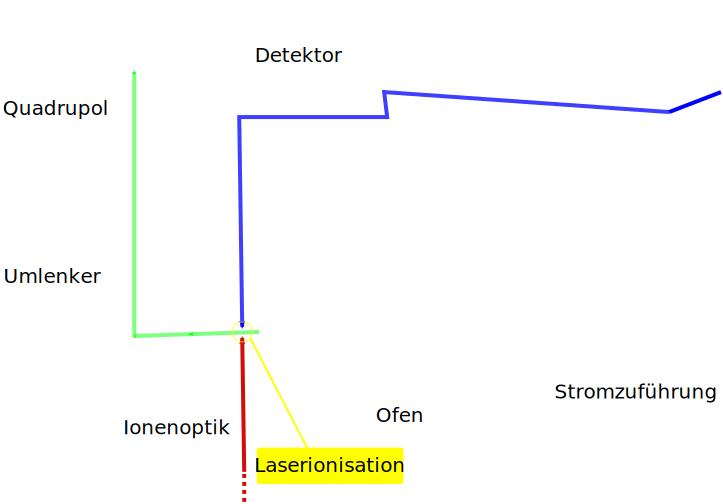
\includegraphics[width=\textwidth-0.3cm]{gfx/vakuumapparatur_foto}
	    }}
	\caption[Vakuumapparatur]{Im Foto ist die verwendete Vakuumapparatur zu sehen.
	Eingezeichnet sind Atom- bzw. Ionenstrahl (grün), Laserstrahlen (blau und rot),
	Ofen mit Stromzuführung, Wechselwirkungsregion, Ionenoptik, Umlenker,
	Quadrupol und Detektor.}\label{fig:vakuumapparatur_foto}
\end{figure}
Rechts befindet sich der Atomstrahlofen, der aus einem $50\,$mm langem
Graphitröhrchen mit einem (Innen-)Durchmesser von ($2,9\,$mm) $4,1\,$mm besteht \cite{raeder:2006:diplomarbeit}. Das Röhrchen lässt sich einseitig auf einen
Molybdänstab schrauben, der gleichzeitig als Stromzuführung dient. Die andere
Seite des Röhrchens ist mit der zu untersuchenden Uran-Probe befüllt und wird
leicht gegen eine kleeblattförmige Blende gedrückt, die als stromabführung dient. Alle
stromführenden Bauteile sind aus Kühlzwecken entweder wasserdurchflossene
Kupferblöcke oder werden von solchen umgeben. Der Ofen kann bei einem Strom von
maximal $120\,$A bis auf $2300\,$K aufgeheizt werden. Der Ofen
befindet sich momentan im Entwicklungsstadium, sodass sich die
Konfiguration in nächster Zeit teilweise ändern wird.\par
Der durch das Aufheizen der Probe nach links austretende Atomstrahl durchläuft
die Wechselwirkungszone mit den Lasern, in der durch Resonanzionisation
Laserionen erzeugt werden. Die Laser werden dabei transversal zum Atomstrahl
und wegen der Dopplerkompensation gegenläufig eingestrahlt. Die Ionen werden
mithilfe einer Ionenoptik transportiert, über einen 90°-Quadrupolumlenker in das
QMS geführt und anschließend mit einem Kanalelektronenvervielfacher
(Channeltron) detektiert.
Ionen, die ungewollt vor der Wechselwirkungszone mit den Lasern entstanden sind
(sog.
Oberflächenionen) werden mithilfe einer Repellerlinse, die auf positivem
Potential relativ zum Ofen liegt, abgeblockt.
So erreicht man bei ausgeschalteten Lasern eine Dunkelzählrate in der
Größenordnung von $10^{-3}$ Ionen pro Sekunde.\par
Das QMS, auf das im folgenden Abschnitt \ref{subsec:quadrupolmassenspektrometer}
etwas näher eingegangen wird, filtert alle Teilchen außer die eines bestimmten
Masse-Ladungs-Verhältnisses aus. In der hochselektiven
Resonanzionisationsspektroskopie ist dies auf den ersten Blick nicht nötig, da nach der Wechselwirkungregion nur noch Laserionen des Zielisotops weiter in das QMS geleitet werden, was auch
näherungsweise zutrifft. Das QMS stellt jedoch sicher, dass weder Ionen
eines falschen Isotops, noch Ionen des Restgases, des Ofenmaterials oder ionische
Moleküle anderer Massen detektiert werden. Diese können durch Konkurenzprozesse,
z.B. Stöße oder nichtresonante Photoionisation entstehen.

\subsection{Quadrupolmassenspektrometer}\label{subsec:quadrupolmassenspektrometer}
\begin{figure}[h]
 	\centering
 	\fbox{\parbox{\dimexpr \linewidth - 2\fboxrule - 2\fboxsep}{
 	\centering
	    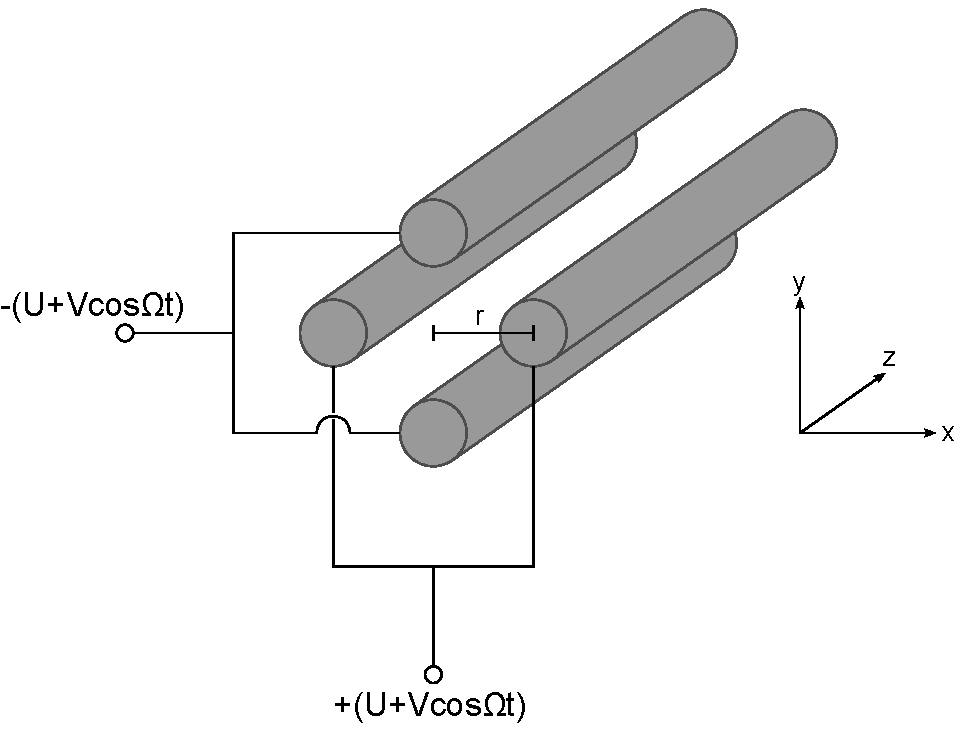
\includegraphics[width=\textwidth-4cm]{gfx/quadrupolmassenspektrometer}
	    }}
	\caption[Quadrupolmassenspektrometer,
	schematisch]{Die Zeichnung zeigt den schematischen Aufbau eines
	Quadrupolmassenspektrometers mit runder
	Stabgeometrie.}\label{fig:quadrupolmassenspektrometer}
\end{figure}
Ein QMS besteht aus vier äquidistant radial angeordneten runden
Metallstäben mit Abstand $r$ zum Zentrum, wie in
\ref{fig:quadrupolmassenspektrometer} schematisch dargestellt ist. Zwei
gegenüberliegende Stäbe haben jeweils immer dasselbe Potential
\begin{equation}\label{eq:qms_potential_0}
	\Phi_0(t)=\pm\left(U+V\cos{(\Omega t)}\right)\,.
\end{equation}
Das Potential $\Phi_0(t)$ setzt sich aus einer konstanten Spannung $U$
und einer Wechselspannung $V\cos{(\Omega t)}$ mit der Frequenz $\Omega=1,2\,$MHz
zusammen. Zwischen den Stäben ergibt sich das ortsabhängige Potential
\begin{equation}\label{eq:qms_potential_ort}
	\Phi_0(\vec{r},t)=\pm\left(U+V\cos{(\Omega
	t)}\right)\cdot\frac{x^2-y^2}{r^2}\,,
\end{equation}
das konstant in z-Richtung ist. Aus der Bewegungsgleichung
\begin{equation}\label{eq:qms_bewegungsgleichung}
	m\ddot{\vec{r}}+e\vec{\nabla}\Phi(\vec{r},t)
\end{equation}
ergeben sich die \textit{Mathieu'schen Differentialgleichungen}
\begin{subequations}\label{eq:qms_mathieu}
	\begin{equation}\label{eq:qms_mathieu_01}
		\fracdd{x}{\xi}+(a_x+2q_x\cdot\cos{2\xi})\cdot x=0
	\end{equation}
	\begin{equation}\label{eq:qms_mathieu_02}
		\fracdd{y}{\xi}-(a_y+2q_y\cdot\cos{2\xi})\cdot y=0
	\end{equation}	
\end{subequations}
mit den Transformationsparametern
\begin{subequations}\label{eq:qms_mathieu_trsf}
	\begin{equation}\label{eq:qms_mathieu_trsf_01}
		\Omega t=2\xi
	\end{equation}
	\begin{equation}\label{eq:qms_mathieu_trsf_02}
		a_x=-a_y=\frac{8eU}{mr^2\Omega^2}
	\end{equation}
	\begin{equation}\label{eq:qms_mathieu_trsf_03}
		q_x=-q_y=\frac{4eV}{mr^2\Omega^2}\,.
	\end{equation}
\end{subequations}
Ohne die exakten mathematischen Lösungen der Differenzialgleichungen herzuleiten
soll die Lösung hier nur qualitativ diskutiert werden. Die Lösungen der
DGLn können in zwei Klassen eingeteilt werden: stabile und instabile Lösungen.
Die Lösung für Teilchen mit dem Ladungs-Masseverhältnis $\nicefrac{e}{m}$,
die den Quadrupol passieren und vom Detektor registriert werden können, nennt
man stabil.
Alle anderen Lösungen sind instabil.
Trägt man nun die Parameter $a$ und $q$ gegeneinander auf, findet man in erster
Ordnung das Stabilitätsdiagramm aus Abb.
\ref{fig:stabilitaetsdiagramm}\subref{subfig:stabilitaetsdiagramm_aq}.
\begin{figure}[h]
	\centering
	\fbox{\parbox{\dimexpr \linewidth - 2\fboxrule - 2\fboxsep}{
	\subfloat[]{
		\label{subfig:stabilitaetsdiagramm_aq}
		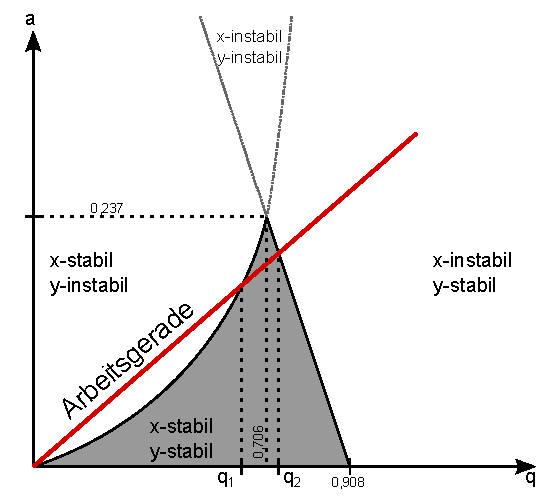
\includegraphics[width=(\textwidth-1cm)/2]{gfx/stabilitaetsdiagramm_aq}
  	}
	\subfloat[]{
		\label{subfig:stabilitaetsdiagramm_UV}
		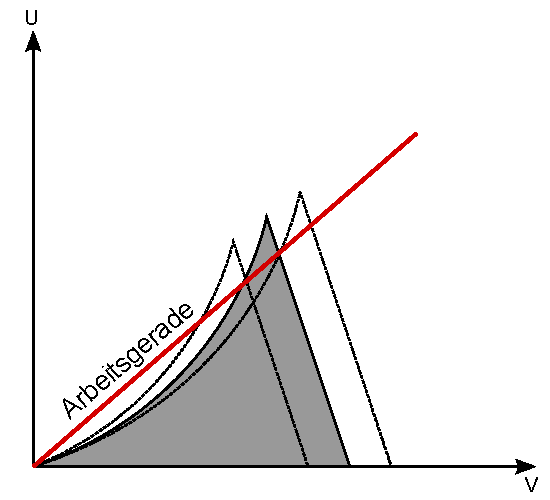
\includegraphics[width=(\textwidth-1cm)/2]{gfx/stabilitaetsdiagramm_UV}
  	}
	}}
	\caption[Stabilitätsdiagramm]{In (a) ist in grau das Stabilitätsdiagramm erster
	Ordnung in Abhängigkeit von den Parametern $a$ und $q$ eingezeichnet. Die
	gestrichelten Dreiecke in (b) sind die stabilen Bereiche von Teilchen mit
	anderen $\nicefrac{e}{m}$-Verhältnissen ($U$-$V$-Abhängigkeit).}
	\label{fig:stabilitaetsdiagramm}
\end{figure}
%TODO: Stabilitätsdreieck nicht so steil
Nur die Teilchen, deren $a$ und $q$ im grauen
Bereich liegen, sind sowohl in x- als auch in y-Richtung stabil und werden nicht
ausgefiltert. Rechts davon sind diese Teilchen in x-Richtung instabil und in
y-Richtung stabil. Umgekehrtes gilt für den Bereich links oberhalb dieses
Gebiets.
Oberhalb der Spitze des Dreiecks sind die Lösungen in beide Dimensionen
instabil.
Der Quotient $\nicefrac{a}{q}=\nicefrac{2U}{V}$ ist unabhängig von dem
Ladungs-Masseverhältnis der Teilchen und bildet die Steigung für die
in Abb. \ref{fig:stabilitaetsdiagramm} eingezeichnete Arbeitsgerade. Die
Einstellung dieses Quotienten wirkt sich auf das Masseintervall $\Delta m=[m_1,m_2]$ aus, was
gleichbedeutend mit dem Intervall $[q_1,q_2]$ ist, in dem Transmission auftritt.
Je schärfer die Arbeitsgerade die Spitze des Stabilitätsdreiecks schneidet desto besser ist die Massenauflösung
$R=\nicefrac{m}{\Delta m}$. Die gestrichelten Stabilitätsdreiecke in
\ref{fig:stabilitaetsdiagramm}\subref{subfig:stabilitaetsdiagramm_UV}
($U$-$V$-Raum) entsprechen denjenigen Teilchen mit anderen
$\nicefrac{e}{m}$-Verhältnissen entsprechend benachbarter Massen, wenn man davon
ausgeht, dass alle Ionen einfach positiv geladen sind.
Mit einem simultanen Verfahren von $U$ und $V$ bei Beibehalten des Verhältnisses
$\nicefrac{2U}{V}$ können die Spitzen der Stabilitätsdreiecke von Teilchen verschiedener Masse angefahren und die entsprechenden Teilchen
selektiert werden. Streng genommen liegen die Spitzen der
Stabilitätsdreiecke nicht auf einer Geraden, sondern auf einem Polynom höheren
Grades. Deshalb wäre es nötig, den Quadrupol für verschiedene Massenbereiche
einzeln zu kalibrieren. Da zur Untersuchung der Uranisotope aber nur ein sehr
begrenztes Massenintervall nötig ist ($^{233}$U bis $^{238}$U), reicht eine
einmalige Kalibration für diesen Bereich.\par
Der hier verwendete QMS von der Firma \textit{ABB
Extrel} ist ausgelegt für einen Massenbereich von $0\,$-$300\,$u. Die Massen
können durch ein Modulationsspannungssignal (\textit{Masscommand}) über einen
DAC von einem PC aus angefahren werden. Bis zum Ende dieser Arbeit wurde diese
Möglichkeit für das neue System noch nicht implementiert. Alternativ wird
hierfür ein PC des alten Systems verwendet. Massenscans im Zusammenhang mit der
Messdatenaufnahme des neuen Systems sind daher noch nicht möglich, sollen aber
im Anschluss an diese Arbeit nachgerüstet werden.

\section{Messdatenverarbeitung}\label{sec:messdatenverarbeitung}
In diesem Abschnitt soll kurz die Verarbeitung des Ionensignals beschrieben
werden. Die selektierten Ionen treffen nach dem QMS auf einen
Kanalelektronenvervielfacher, der sensitiv auf einzelne Teilchen ist. Durch das
Eintreffen eines einzelnen Primärteilchens werden durch eine Konversionsdynode
Sekundärelektronen ausgelöst, die über mehrere Kaskaden im Trichter des
Kanalelektronenvervielfachers eine Elektronenlawine in der Größenordnung von
$10^8$ Elektronen auslösen. Der Elektronenstrom wird über einen Verstärker an
einen Diskriminator weitergeleitet, der mithilfe eines Komparators einen
TTL-Puls pro detektiertem Teilchen erzeugt.\par
Ein 32-Bit-Counter \cite{counterkarte_countraten}, welcher aus einer
anderen, früheren Anwendung stammt, zählt die Ereignisse und stellt die
Countraten in voreinstellbaren Intervallen von $0.1$ bis $10\,$s über eine SPI-Schnittstelle in 4x8-Bit Datenpaketen zur Verfügung. Das SPI-Protokoll bietet die Möglichkeit einer Kommunikation
zwischen beliebig vielen Mikrocontrollern, wobei ein Mikrocontroller die Rolle
des Masters übernimmt, während alle anderen im Slave-Modus betrieben werden.
Hier ist der Mikrocontroller \textit{MEGA16-P} des Counters Master und ein
\textit{Arduino} Slave. Der \textit{Arduino} berechnet aus den 4x8-Bit Datenpaketen die Countrate
und leitet diese über eine RS232-Schnittstelle an den PC weiter (siehe Kap.
\ref{kap:software}).

\section{Vergleich mit altem System}\label{sec:vergleich_mit_altem_system}
In diesem Abschnitt sollen kurz die Unterschiede zu dem bisher genutzten
Lasersystem aufgezeigt werden. Das alte System besteht aus drei in Mainz
entwickelten Diodenlasern. Der Laser des ersten Anregungsschritts ist eine
$415\,$nm-Diode. Sie stammt aus den Entwicklungszeiten
der \textit{BluRay}$^\text{\textregistered}$-Laufwerke und ist nun nicht mehr
erhältlich. Die im finalen Entwicklungsstatus der \textit{BluRay}-Technik
verwendeten Laserdioden haben eine Wellenlänge von $405\,$nm. Aufgrund der
Annahme, dass die Liquidität der \textit{BluRay}-Laufwerke auf dem Markt noch
einige Jahre anhält, wird im neuen Laser eine $405\,$nm-Lasediode verwendet.
Nachteil dabei ist, dass neue Anregungsschemata gefunden werden müssen, wie in Kap.
\ref{kap:charakterisierung} diskutiert wird. Die Laser des zweiten und
dritten Schritts sind $772\,$nm-Dioden, wobei das Licht des dritten Lasers wie
auch beim neuen System durch einen Trapezverstärker verstärkt wird. Mit diesem
können Leistungen bis $1500\,$mW erreicht werden.\par
Der große Unterschied zum neuen System ist die Stabilisierung der Laser.
Hierbei wurde ausschließlich auf das FOL gesetzt. Es wird ebenfalls
ein geramptes FPI verwendet, das allerdings sowohl im roten als auch im blauen
Bereich eine hohe Finesse hat. Die Signalgenerierung aus den
Transmissionssignalen erfolgt analog zur oben beschriebenen Technik. Die
Counterkarte ist in einem Windows-NT$^\text{\textregistered}$-PC integriert, der
gleichzeitig für die Stabilisierung zuständig ist. Die Software für die Regelung
ist aufgrund der zeitkritischen Berechnungen auf Treiber-Ebene
geschrieben. Über direkt an den PC angeschlossene DACs werden die Parameter der
Laser (Diodenstrom und Piezospannung) moduliert. Parallel zur Regelung läuft auf
der Anwendungsebene ein Serverprogramm, das Monitoring-Aufgaben übernimmt und
Befehle von einem über TCP-IP verbundenen Client entgegennimmt. Die
Clientsoftware kann auf einem beliebigen Rechner im Netzwerk laufen und dient
als Benutzerinteraktionsschnittstelle.\par
Die alleinige Nutzung des FOL macht die Implementierung des
alten Systems wesentlich einfacher. Die erhofften Vorteile des neuen,
komplizierteren "`Hybrid"'-Systems aus \textit{iScan} und FOL
sind eine Erhöhung der Kurzzeitstabilität, eine geringere Rate an Frequenzfehlmessungen
und schnelleres Scannen über große Frequenzbereiche. Weiterhin werden im neuen
System zwei kommerzielle, wesentlich stabilere Diodenlaser im zweiten und
dritten Anregungsschritt verwendet. Zusammenfassend wird damit eine höhere
Stabilität und eine geringere Zählratenfluktuation erwartet. Tabelle
\ref{tab:vergleich_alt_neu} stellt nochmal einen Vergleich beider Lasersysteme
in Stichpunkten dar.
\begin{table}
	%Summe der Breiten muss 0.91 mal \textwidth sein.
	\begin{tabular}{p{0.31\textwidth}|p{0.30\textwidth}p{0.30\textwidth}}
		\toprule
		Eigenschaft & altes System & neues System\\
		\midrule[1px]
		\hline
		1. Anregungsschritt & $415\,$nm (Eigenbau) & $405\,$nm (Eigenbau)\\
		2./3. Anregungsschritt & $772\,$nm (Eigenbau) & $772\,$nm (kommerziell)\\
		Stabilisierung & FOL & FOL +
		\textit{iScan}\\
		\bottomrule[1px]
	\end{tabular}
	\caption[Vergleich von altem und
	neuem Lasersystem]{Die Tabelle stellt einen Vergleich zwischen altem und neuem
	System dar.}
	\label{tab:vergleich_alt_neu}
\end{table}
%TODO: !!Vergleichstabelle ausführlicher
